\chapter{Simulation model}
\label{chap:simulation_model}

\section{General structure}

The model is developed in Python and consists of two classes (see fig. \ref{uml}) : the HydropowerPlant class, which represents a run-of-the-river power plant and the Modelchain class which represents the simulation of on plant. The attributes and methods of each class are detailled in table \ref{att_meth}.
\begin{figure}[H]
\center
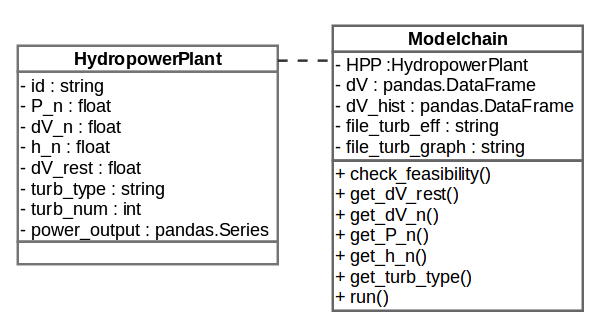
\includegraphics[width=10cm]{uml.png}
\caption{Classes of the hydropower model}
\label{uml}
\end{figure}

\begin{table}
\footnotesize
 \caption{Attributes and methods of the classes}
 \centering
 \label{att_meth}
 \begin{tabular}{|l|l|l|p{7cm}|}
  \cline{2-4}
  \multicolumn{1}{c|}{}&\multicolumn{3}{c|}{\textbf{class HydropowerPlant}}\\ \hline
  \multirow{8}{*}{\rotatebox[origin=c]{90}{\textbf{Attributes}}}&id&string&Identification of the plant\\
  &P{\_}n&float&Nominal power of the plant in \unit{W}\\
  &dV{\_}n&float&Nominal water flow of the plant in \unit{m\textsuperscript{3}\textperiodcentered s\textsuperscript{-1}}\\
  &h{\_}n&float&Nominal head of water in \unit{m}\\
  &dV{\_}rest&float&Residual water flow in \unit{m\textsuperscript{3}\textperiodcentered s\textsuperscript{-1}}\\
  &turb{\_}type&string&Type of turbine(s)\\
  &turb{\_}num&int&Number of turbines. Default : 1\\
  &power{\_}output&pandas.Series&Power output in \unit{W}\\
  \hline
  \multicolumn{1}{c|}{}&\multicolumn{3}{c|}{\textbf{class Modelchain}}\\ \hline
  \multirow{5}{*}[-1cm]{\rotatebox[origin=c]{90}{\textbf{Attributes}}}&HPP&HydropowerPlant&Plant to simulate\\
  &dV&pandas.DataFrame&Runoff time series in \unit{m\textsuperscript{3}\textperiodcentered s\textsuperscript{-1}} with DateTime index over the period to simulate\\
  &dV{\_}hist&pandas.DataFrame&Runoff time series in \unit{m\textsuperscript{3}\textperiodcentered s\textsuperscript{-1}} with DateTime index over several past years\\
  &file{\_}turb{\_}eff&string&File containing parameters about the turbine efficiency\\
  &file{\_}turb{\_}graph&string&File containing the characteristic diagrams\\
  \hline
  \multirow{7}[5]{*}{\rotatebox[origin=c]{90}{\textbf{Methods}}}&check{\_}feasibilty()&boolean&Checks if input data is sufficient \\
  &get{\_}dV{\_}rest()&float&Calculates residual runoff value in \unit{m\textsuperscript{3}\textperiodcentered s\textsuperscript{-1}}\\
  &get{\_}dV{\_}n()&float&Calculates HPP.dV{\_}n in \unit{m\textsuperscript{3}\textperiodcentered s\textsuperscript{-1}}\\
  &get{\_}P{\_}n()&float&Calculates HPP.P{\_}n in \unit{W}\\
  &get{\_}h{\_}n()&float&Calculates HPP.h{\_}n in \unit{m}\\
  &get{\_}turb{\_}type()&string&Finds type of turbine\\
  &run()&void&Calculates HPP.power{\_}output in \unit{W}\\
  \hline
 \end{tabular}
\end{table}


\section{Implementation details}
\section{Results post-processing}
